\documentclass{../cssheet}

%--------------------------------------------------------------------------------------------------------------
% Basic meta data
%--------------------------------------------------------------------------------------------------------------

\title{Aufgaben für Entdecker*innen}
\author{Prof. Dr. Christian Spannagel}
\date{\today}
\hypersetup{%
    pdfauthor={\theauthor},%
    pdftitle={\thetitle},%
    pdfsubject={Aufgabenblatt Inside Math!},%
    pdfkeywords={insidemath}
}

%--------------------------------------------------------------------------------------------------------------
% document
%--------------------------------------------------------------------------------------------------------------

\begin{document}
\printtitle

\vspace*{10mm}

\textbf{Vorbemerkung:}  In den folgenden Aufgaben geht es darum, Muster zu finden und zu begründen, dass man ein korrektes Muster gefunden hat. Findet ihr die Muster? Wie könnt ihr dabei vorgehen? Welche Strategien setzt ihr ein? Und könnt ihr begründen, dass das Muster korrekt ist? Wie? Die Aufgaben dienen also unter anderem dazu, dass ihr euch bewusst macht, welche Techniken und Strategien ihr beim Lösen solcher Aufgaben einsetzen könnt. Macht euch eine Liste aller Strategien!


\textbf{Aufgabe 1 (Drillinge):}  Schaut euch einmal die folgenden Rechnungen an. Könnt ihr ein Muster erkennen? Welches? Und könnt ihr es begründen?

\begin{itemize}
\item $3+4+5$
\item $7+8+9$
\item $59+60+61$
\item $111+112+113$
\item \ldots
\end{itemize}

\textbf{Aufgabe 2 (Schon wieder\ldots):} Macht dasselbe wie in Aufgabe~1 mit folgenden Rechnungen:

\begin{itemize}
\item $1\cdot3 + 1$
\item $2\cdot4 + 1$
\item $3\cdot5 + 1$
\item $4\cdot6 + 1$
\item \ldots
\end{itemize}

\textbf{Aufgabe 3 (Erbsenstapelei):} Beim Stapeln von Erbsen gilt es, bestimmte Formen einzuhalten. Aus wie vielen Erbsen besteht jeweils die $5.$, $6.$, …, $10.$, …, $20.$ Erbsenform? Entdeckt ihr eine Regelmäßigkeit? Aus wie vielen Erbsen besteht die $1000.$ Form?

\begin{center}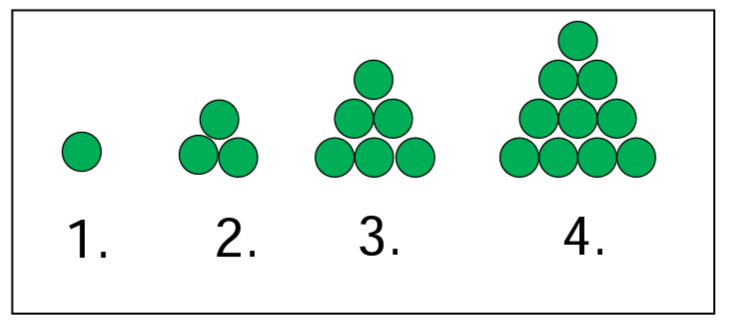
\includegraphics[width=10cm]{erbsen.png}\end{center}

%\vspace*{10mm}
\newpage
\printlicense

\printsocials

\end{document}
